\documentclass[review]{elsarticle}

\usepackage{lineno,hyperref}
\modulolinenumbers[5]

\journal{Journal of Computers and Fluids}

%% `Elsevier LaTeX' style
\bibliographystyle{elsarticle-num}
\usepackage{caption}
\usepackage{subcaption}
\usepackage{amsmath}
%%%%%%%%%%%%%%%%%%%%%%%

\begin{document}

\begin{frontmatter}

\title{Auto-tuned Jacobi-like Multi-grid Smoother\\ for Fast Pressure Projection}

%% Group authors per affiliation:
\author{Gabriel D Weymouth}
\address{Engineering and Physical Sciences, University of Southampton, Southampton, UK}
\address{Data-Centric Engineering, Alan Turing Institute, London, UK}
\ead[url]{https://weymouth.github.io/}

\begin{abstract}
Pressure projection is the single most computationally expensive step in an unsteady incompressible fluid simulation. This work discusses the potential of data-driven methods to accelerate the approximate solution of the Poisson equation at the heart of pressure projection, linking Multigrid methods to Convolutional Neural Networks. Required to maintain linearity in pressure, the best option for data-driven acceleration is in the smoothing step. Using automatic differentiation, a high-speed parameterized smoother is developed which outperforms classic Multi-grid methods by 66-200\% on eleven 2D and 3D benchmarks. The tuned parameters are found to transfer nearly 100\% effectiveness as the resolution is increased, providing a robust approach for accelerated pressure projection of any flow.
\end{abstract}

\begin{keyword}
pressure projection, linear algebra, data-driven
\end{keyword}

\end{frontmatter}

\section{Introduction}

Pressure projection is a bottleneck in high-speed unsteady incompressible flow solvers. Constructing approximate solutions the discrete pressure Poisson system typically makes up 25-50\% of the solution cost even in serial simulations, and the proportional cost grows in massively parallel simulations as the elliptic equation requires communication throughout the computational domain instead of being confined to a local characteristic. Methods such as artificial-compressibility, smooth-particle-hydrodynamics, and particle-in-cell attempt to side-step this computational cost by modelling or otherwise under-resolving the pressure evolution compared to the fluid's momentum. However, these approaches lead to significant errors in pressure forces, thereby making them unsuitable for many applications or requiring explicit pressure corrections.

Recent advances in data-driven acceleration of flow solvers have mainly focused on data-assimilation methods and data-driven turbulence closures. Data-assimilation methods typically avoid the expensive pressure projection step entirely, focusing on applications where time-accurate pressure forces are not important. Data-driven closures for Large Eddy Simulation (LES) and Unsteady Reynolds Averaged Navier-Stokes (unRANS) and even Spanwise Averaged Navier-Stokes (SANS) simulations have seen growing success and are capable of accurate force prediction. Deep learning Convolutional Neural Networks (CNN) have enabled many of these turbulence closures as well as other fluids applications such as super-resolution and generative models. CNN architectures have inherent translational symmetry and often use a restriction phase, where the size of the network is reduced before expanding again, both of which help generalize the trained networks to unseen prediction cases. 

However, none of these studies have applied data-driven techniques to accelerate the critical projection step itself. Some recent work has focused on the pressure projection step explicitly. Chaotic projection methods for massively parallel systems; not data driven. Multi-grid data-driven decomposition; high errors and unclear speed-up. This work develops a high-speed data-driven project method which outperforms classic methods on eleven 2D and 3D benchmarks. Moreover, as the approach in linear in the pressure and scale-invariant, the parameters can be tuned on a coarse simulation and maintain their accelerated performance on unseen fine-grid simulations. 

\section{Linear System Description}

The discrete Poisson equation in the projection step is defined as
\begin{equation}\label{eq:axb}
    A x = b
\end{equation}
where $x$ is the desired pressure field vector, $b$ is the source term (proportional to the divergence of the velocity field to be projected), and $A$ is the Poisson matrix. For conservative Poisson equations, $A$ is symmetric, has zero-sum rows and columns, is negative semi-definite, and has a single zero eigenvalue. The matrix is also extremely sparse. Using a second-order scheme on structured grids in $M$ dimensions, $A$ has only $M$ non-zero sub-diagonals. While the solution vector size $N$ may easily be larger than $10^6$, the matrix-vector multiplication $Ax$ only has computational cost $O(NM)=O(N)$ instead of $O(N^2)$.

Iterative methods solve equation \ref{eq:axb} by updating an approximate solution $x^k$ to a new solution $x^{k+1}$ with reduced error. As the problem is linear, the equation for the update $\epsilon$ is simply
\begin{equation}\label{eq:aer} 
    A \epsilon^k = r^k \equiv b - Ax^k
\end{equation}
where $r$ is the residual. In practise, only an approximate solution for $\epsilon$ is obtained, after which the solution and residual are incremented
\begin{equation}
    x^{k+1} = x^k+\epsilon^k, \quad r^{k+1} = r^k-A\epsilon^k.
\end{equation}
This process is iterated until the residual is reduced sufficiently, the required tolerance level being highly dependant on the application.

Multi-grid (MG) methods are among the fastest iterative solution approaches for variable coefficient discrete pressure Poisson equations. The MG operator is effectively a \textit{linear} convolutional architecture where the system is preconditioned before the residual is restricted down to a reduced-size problem and the correction is prolongated back up. 
% \begin{equation}
%     r_c = R r \quad\rightarrow\quad A_c \epsilon_c = r_c \quad\rightarrow\quad \epsilon = P \epsilon_c
% \end{equation}
% where $R$ is the $N_c \times N$ restriction operator, $P$ is the $N \times N_c$ prolongation operator 
The restriction-solve-prolongation process, a V-cycle, distributes the residual throughout the domain, which enables simple and relatively fast stationary methods such as Gauss-Sidel or Successive Over Relation (SOR) to \textit{smooth} the local high-frequency error in the projected solution. The MG architecture proceeds recursively on the reduced-size problems until a small linear algebra problem is reached which can be approximated with minimal cost. This recursive approach results in only $O(N\log N)$ computational cost.

\section{Data-driven Accelerated Solution Methods}

As \textit{any} element of the residual of the elliptic system potentially influences \textit{every} element of the update, $O(N\log N)$ is the best possible solution time scaling. However, data-driven methods can still be used to accelerate pressure projection methods by speeding-up and increasing the residual reduction of each V-cycle iteration.

The linearity of equation \ref{eq:aer} is a critical property which the data-driven method must maintain in order to be useful in practise, but this linearity is only with respect to the update and residual fields. The operators of the ``MG network'' can all potentially be optimized for a specific sub-class of problems. In particular, those operators can be made into parameterized nonlinear functions of $A$, embedding information about the discrete problem and boundary conditions. 

Which MG operation is the best candidate for such an approach? The prolongation operator (restriction simply being its transpose) is not inherently a function of $A$, and while related super-resolution operators have seen improvements in the literature, these are always nonlinear functions of the field. The precondition operator is an option, but a simple Jacobi preconditioner
\begin{equation}
    \epsilon = D^{-1}r
\end{equation}
where $D$ is the diagonal of $A$, is as fast as possible and is sufficient for the V-cycle to distribute the residual throughout the domain. Therefore, for the remainder of the paper we will focus on the smoother as the best candidate for acceleration, using a simple Jacobi preconditioner and uniform pooling/distribution for restriction/prolongation.

While more complex options are certainly possible, this work uses a simple parameterized Jacobi-like smoother
\begin{equation}
    \epsilon = \tilde A^{-1}r
\end{equation}
where $\tilde A^{-1}=f(A\,|\theta)$ is an approximate matrix-inverse with the same sparsity as $A$ and parameter vector $\theta$. 
%The matrix $A$ is constant during the projection step (and often for an entire simulation), meaning $\tilde A^{-1}$ can be computed and stored ahead of time.
Unlike Gauss-Sidel or SOR smoothers, the matrix-vector multiplication smoother requires no back-propagation and so can be vectorized in serial or parallel implementations, offering a significant potential speed-up.

There are few constraints on $\tilde A^{-1}$: it must have units of $A^{-1}$, and symmetry of $A$ implies the approximate inverse should also be symmetric. For simplicity, the diagonal and off-diagonal coefficients of $\tilde A^{-1}$ are constructed independently 
\begin{equation}
    \tilde a^{-1}_{ii} = \frac{f_d(a_{ii}/s\,|\theta_d)}{a_{ii}} , \quad
    \tilde a^{-1}_{ij} = \frac{f_o(a_{ij}/s\,|\theta_o)}{a_{ii}+a_{jj}}
\end{equation}
where function inputs are scaled by the maximum off-diagonal $s=\max(A-D)$ and the outputs are scaled by the diagonal elements. Note a Jacobi smoother would use a diagonal function $f_d=1$ and off-diagonal function $f_o=0$. With the learning problem now reduced to two normalized single-variable functions, the specific choice of parameterization is not critical and a simple quadratic polynomial $f(a) = \sum_{p=0}^2 a^p \theta_p$ is chosen for $f_o$ and $f_d$. Using higher-order polynomials, splines, and interpolating kernels did not significantly change the results.

Automatic differentiation (AD) is used to optimize the parameterized smoother for a set of training data $X=\{A,x^k,b\}$. The loss function is simply the reduction in the norm of the residual after a V-cycle iteration $L = \log_{10}(|r^{k+1}| / |r^{k}|)$, which means that example pressure \textit{solutions} are not required. This loss is averaged over each iteration and each example in the data-set. The optimal parameters are defined as
\begin{equation}
    \hat\theta = \min_\theta L(\theta\, |X)
\end{equation}
and determined using Newton's method. The ForwardDiff.jl AD package is used determine the gradient $\nabla_\theta L$ and Hessian $H_{\theta\theta} L$ automatically, avoiding inaccurate and potentially unstable finite differences of the nonlinear recursive loss function.

\begin{figure}
    \centering
    \begin{subfigure}[b]{0.3\textwidth}
        \centering
        \caption{2D-box}
        \label{fig:2D-box}
    \end{subfigure}
    \begin{subfigure}[b]{0.3\textwidth}
        \centering
        \caption{2D-$\mu$}
        \label{fig:2D-mu}
    \end{subfigure}
    \begin{subfigure}[b]{0.3\textwidth}
        \centering
        \caption{2D-sphere}
        \label{fig:2D-sphere}
    \end{subfigure}
    \begin{subfigure}[b]{0.47\textwidth}
        \centering
        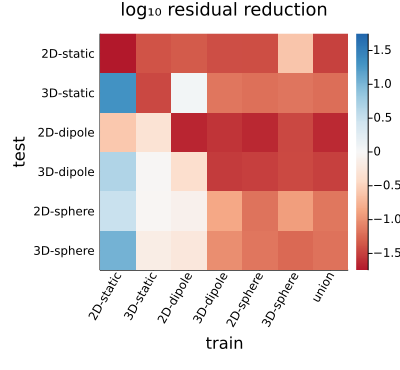
\includegraphics[width=\textwidth]{figures/crossloss.png}
        \caption{single-cycle residual reduction}
        \label{fig:cross plot}
    \end{subfigure}
    \hfill
    \begin{subfigure}[b]{0.47\textwidth}
        \centering
        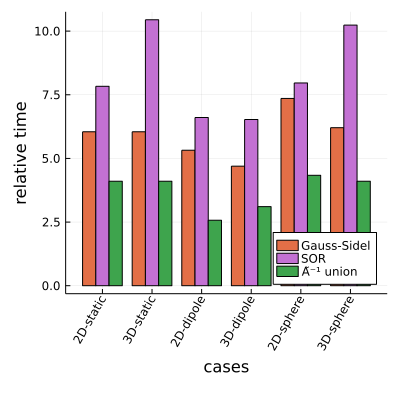
\includegraphics[width=\textwidth]{figures/synthetic_timing.png}
        \caption{solver time}
        \label{fig:synthetic time}
    \end{subfigure}
    \caption{(a-c) Sample solutions from the data-sets of three of the six synthetic cases. (d) Residual reduction over a single Multi-grid V-cycle on the `test' cases after tuning using the `train' case. Training case `union' refers to the smoother trained on all of the synthetic cases. (b) Time to reduce pressure residual by $10^{-3}$ for classical and parameterized smoothers on each synthetic case. Time is relative to the time of a single V-cycle using the Jacobi smoother.}
    \label{fig:synthetic cases}
\end{figure}

\section{Synthetic Projection Systems and Results}

A set of six synthetic projection cases were constructed to establish the characteristics of the parameterized smoother. The three 2D cases are shown in Figure~\ref{fig:2D-box}-\ref{fig:2D-sphere}, and each has a matching 3D case. The `static' cases have a hydrostatic gradient throughout the domain, with the direction and magnitude randomized. The `dipole' cases have a localized dipole within a quiescent flow with randomized placement, direction and magnitude. The `sphere' cases have a moving sphere immersed within a quiescent flow with randomized radius, location, and velocity direction. All cases are initialized with $x^0=0$.
%, and all cases feature initially localized residuals; i.e. $r^0\ne0$ only in a fraction of the cells, but $x$ must be updated throughout the domain, starkly illustrating the elliptic nature of the projection step.
Neumann boundary conditions are applied on all boundaries, including the immersed sphere, through adjustment of the $A$ matrix coefficients which are otherwise uniform. 

Figure~\ref{fig:cross plot} characterizes the generalization of the parameterized smoother's residual reduction over a single V-cycle on 100 randomized `test' case examples after optimization using 100 examples of the `train' case. Each example uses a grid size of $n=32^M$ points ($N=32^2$ in 2D and $N=32^3$ in 3D) as testing with other resolutions found essentially no change in the performance. As expected, the performance is best when testing and training on the same case, with a single V-cycle reducing the residual from $10^{-1.17}$ on the 2D-sphere case down to $10^{-1.58}$ on the 3D-box case. While the performance for the simplest cases generalizes poorly, the 2D-sphere smoother generalizes essentially as well as the `union' smoother trained on all of the data. 
%The performance of the `union' smoother is only 1-4\% lower than the smoother trained on the test case for the dipole and sphere cases.

Finally, the acceleration of the `union' data-driven smoother is evaluated on new example data of a different size, $n=64^M$ points. Figure~\ref{fig:synthetic time} shows the time to reduce the residual of each case by $10^{-3}$ relative to the time to run a single V-cycle using a Jacobi smoother, but the results for the Jacobi smoother are not shown since hundreds or even thousands of V-cycles are required to converge. Remarkably, the Jacobi-like parameterized smoother is only around 33\% slower per V-cycle, and yet converges in only 1-3 V-cycles in all cases. This results in a 80-175\% speed-up relative to optimized serial Gauss-Sidel and SOR smoothers. This speed-up will be even more favorable in parallel computation as the new smoother operates directly on the local residual without back-propagation, eliminating any need for additional communication.

\begin{figure}
    \centering
    \begin{subfigure}[b]{0.3\textwidth}
        \centering
        \caption{circle flow}
        \label{fig:circle}
    \end{subfigure}
    \begin{subfigure}[b]{0.3\textwidth}
        \centering
        \caption{Taylor-Green Vortex}
        \label{fig:TGV}
    \end{subfigure}
    \begin{subfigure}[b]{0.3\textwidth}
        \centering
        \caption{flapping wing}
        \label{fig:donut}
    \end{subfigure}
    \begin{minipage}{0.47\textwidth}
        \begin{subfigure}{\textwidth}
        \centering
        \caption{torus flow}
        \label{fig:donut}
        \end{subfigure}
        \begin{subfigure}{\textwidth}
        \centering
        \caption{swimming shark}
        \label{fig:donut}
        \end{subfigure}
    \end{minipage}
    \hfill
    \begin{subfigure}[b]{0.47\textwidth}
        \centering
        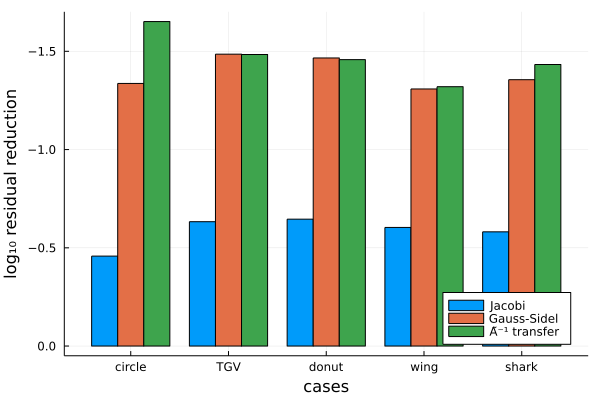
\includegraphics[width=\textwidth]{figures/compareloss.png}
        \caption{single-cycle residual reduction}
        \label{fig:simulation residual}
    \end{subfigure}
    \caption{(a-e) Snapshots from the five flow simulation cases. The Taylor-Green Vortex and torus flow are 3D cases, and the flapping wing and swimming shark have dynamic geometries. (f) Residual reduction over a single Multi-grid V-cycle for classical and parameterized smoothers on each case. The `transfer' smoother has been trained on the union of the synthetic data sets from Figure~\ref{fig:synthetic cases}.}
    \label{fig:simulation cases}
\end{figure}

\section{Unsteady Incompressible Simulation Results}

\begin{figure}
    \centering
    \begin{subfigure}[b]{0.47\textwidth}
        \centering
        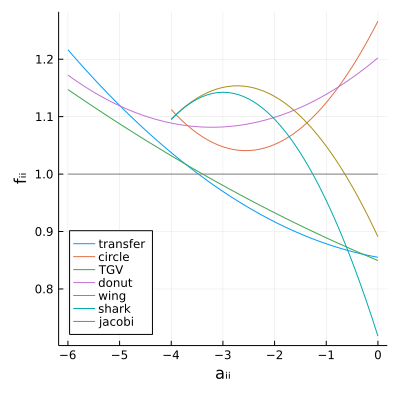
\includegraphics[width=\textwidth]{figures/diag_fun.png}
        \caption{diagonal functions}
        \label{fig:scaled loss}
    \end{subfigure}
    \hfill
    \begin{subfigure}[b]{0.47\textwidth}
        \centering
        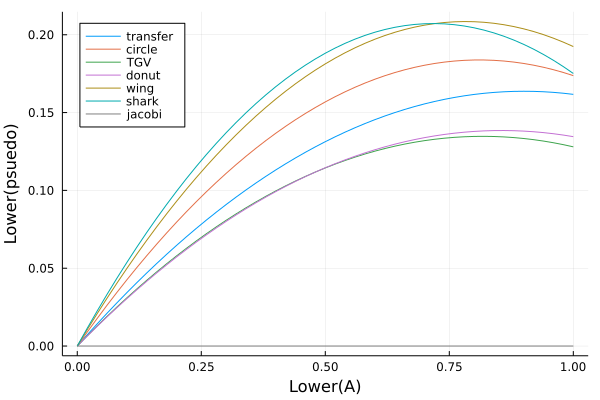
\includegraphics[width=\textwidth]{figures/lower_fun.png}
        \caption{off-diagonal functions}
        \label{fig:simulation time}
    \end{subfigure}
        \caption{(a) Diagonal and (b) off-diagonal parameterized functions after optimization on each simulation case. The `transfer' smoother was tuned on the synthetic cases and `Jacobi' is shown for comparison.}
        \label{fig:tuned simulation}
\end{figure}

\begin{figure}
    \centering
    \begin{subfigure}[b]{0.47\textwidth}
        \centering
        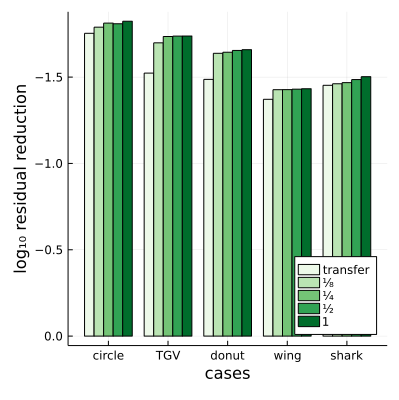
\includegraphics[width=\textwidth]{figures/scaleloss.png}
        \caption{single-cycle residual reduction}
        \label{fig:scaled loss}
    \end{subfigure}
    \hfill
    \begin{subfigure}[b]{0.47\textwidth}
        \centering
        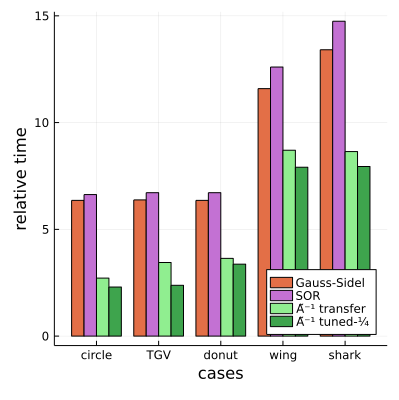
\includegraphics[width=\textwidth]{figures/crosscount.png}
        \caption{solver time}
        \label{fig:simulation time}
    \end{subfigure}
        \caption{(a) Residual reduction over a single Multi-grid V-cycle on the full-resolution case. The `transfer' smoother has been trained on the union of the synthetic data sets from Figure~\ref{fig:synthetic cases}. The $\frac 18, \frac 14, \frac 12$ smoothers have been trained on simulations with the indicated reduced resolution \textit{in each spacial and temporal dimension}. (b) Time to reduce pressure residual by $10^{-3}$ for classical and parameterized smoothers on each simulation case. Time is relative to the time of a single V-cycle using the Jacobi smoother.}
        \label{fig:tuned simulation}
\end{figure}


\section{Conclusions}

\section*{References}

\bibliography{mybibfile}

\end{document}